% ============================================================
% DIAGRAM: BERT Encoder-Only Architecture (2018)
% ============================================================
% Caption: Figure 6.3: BERT encoder-only architecture with bidirectional attention.
%          (Adapted from Devlin et al., 2018, p. 2)
% ============================================================

\documentclass[tikz,border=10pt]{standalone}
\usepackage{tikz}
\usepackage{amsmath}
\usepackage{amsfonts}

\usetikzlibrary{shapes,arrows,positioning,fit,calc,backgrounds}

\begin{document}

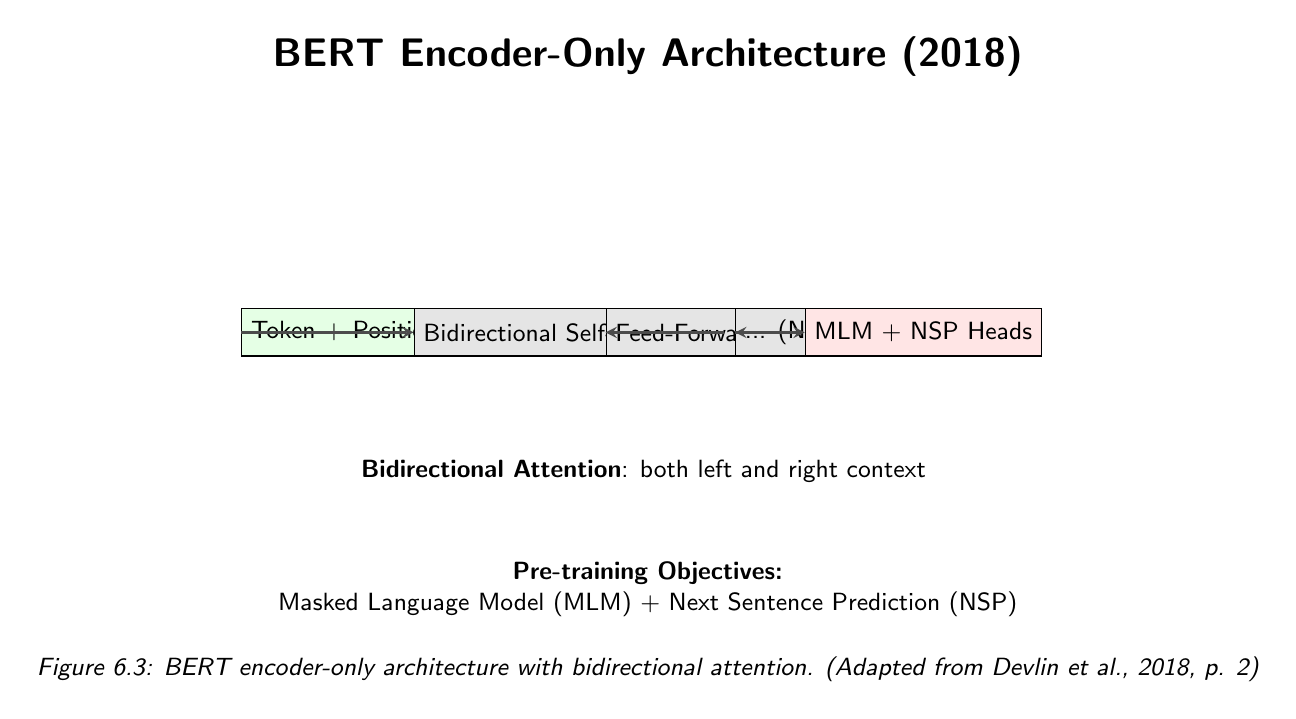
\begin{tikzpicture}[
    block/.style={draw, rectangle, minimum width=0.8cm, minimum height=0.6cm, fill=blue!10, font=\sffamily\small},
    edge/.style={-stealth, thick, draw=black!70},
    label/.style={font=\sffamily\small},
    title/.style={font=\sffamily\Large\bfseries},
    caption/.style={font=\sffamily\small\itshape},
]

\node[title] at (0, 3.5) {BERT Encoder-Only Architecture (2018)};

% Input
\node[block, fill=green!10] (embed) at (-2.5, 0) {Token + Position + Segment Embed};

% Encoder stack (N×)
\node[block, fill=gray!20] (enc1) at (-1, 0) {Bidirectional Self-Attention};
\node[block, fill=gray!20] (enc2) at (0.5, 0) {Feed-Forward};
\node[block, fill=gray!20] (enc3) at (2, 0) {... (N×) ...};

% Output
\node[block, fill=red!10] (out) at (3.5, 0) {MLM + NSP Heads};

\draw[edge] (embed) -- (enc1);
\draw[edge] (enc1) -- (enc2);
\draw[edge] (enc2) -- (enc3);
\draw[edge] (enc3) -- (out);

% Bidirectional
\node[align=center, font=\sffamily\small, anchor=north] at (0, -1.5) {
  \textbf{Bidirectional Attention}: both left and right context
};

\node[align=center, font=\sffamily\small, anchor=north] at (0, -2.8) {
  \textbf{Pre-training Objectives:} \\
  Masked Language Model (MLM) + Next Sentence Prediction (NSP)
};

\node[caption, anchor=north] at (0, -4.0) {
  Figure 6.3: BERT encoder-only architecture with bidirectional attention. (Adapted from Devlin et al., 2018, p. 2)
};

\end{tikzpicture}
\end{document}
